\documentclass[12pt]{article}

\usepackage{sbc-template}
\usepackage{graphicx,url}
\usepackage{longtable}
\usepackage[utf8]{inputenc}
\usepackage[brazil]{babel}
     
\sloppy

\title{
  Aplicação de Algoritmos de \textit{Machine Learning} na previsão de cotação do
  \textit{Bitcoin}
}

\author{
  Rodrigo de Souza Oliveira\inst{1}, 
  Álvaro Viebrantz \inst{1}
}

\address{
  MBA em Big Data -- Fatec – Serviço Nacional de Aprendizagem Industrial (SENAI)\\
  Av. XV de Novembro, 303, Porto - CEP: 78020-300 - Cuiabá–MT
  \email{
    rddsouzaoliveira@gmail.com, 
    emaildoalvaro@gmail.com
  }
}
  
 
\begin{document} 

\maketitle

\begin{abstract}
With the evolution of technology and the creation of several tools for analysis of
data, a subject that has become very relevant is the application of these
advanced Machine Learning techniques to understand the behavior of assets
and subsidize the financial information market for decision making. The objective 
of this work was to apply Machine Learning models, with the goal of
analyze and understand the behavior of bitcoin to forecast its future value
and use it as a tool to assist in investment strategies.
For this, data was collected on the bitcoin quotation through the API of
a crypto exchange, in a historical series created since December 2017.
The results show that the models were able to understand and
forecast bitcoin price fluctuations, highlighting Multilayer
Perceptron model. This work paved the way for a range of possibilities for
future work to better understand model architectures available
that can generalize the behavior of bitcoin over time and to the
development of a tool that automates decision making to operate
in the Bitcoin market automatically.
\end{abstract}
     
\begin{resumo} 
Com a evolução da tecnologia e a criação de diversas ferramentas de análise de
dados, um assunto que vem se tornando muito relevante é a aplicação dessas 
técnicas avançadas de Machine Learning para entender o comportamento dos ativos 
e subsidiar o mercado financeiro de informações para tomada de decisão. Este 
trabalho teve como objetivo aplicar modelos de Machine Learning, com a função de
analisar e entender o comportamento do bitcoin para projetar seu valor futuro 
e utilizá-lo como ferramenta para auxiliar nas estratégiasde investimentos. 
Para isso, foram coletados dados sobre a cotação do bitcoin, através da API de 
uma corretora, em uma série histórica criada desde dezembro de 2017. 
Os resultados evidenciam que os modelos foram capazes de entender e 
projetar as oscilações do preço do bitcoin, com destaque para o Multilayer 
Perceptron. Este trabalho abriu caminho para uma gama de possibilidades de 
futuros trabalhos para melhor entender as arquiteturas de modelos disponíveis 
que consigam generalizar o comportamento do bitcoin ao longo do tempo e o 
desenvolvimento de ferramenta que automatiza a tomada de decisões para operar
no mercado de Bitcoin de forma automática.
\end{resumo}


\section{Introdução}

Investimento é a aplicação de algum recurso, com a expectativa de algum gannho 
futuro. A incerteza do ganho, ou um possível prejuízo, caracteria o risco do
investimeto. No contexto de aplicação financeira, pode-se caracterizar o 
investimento como a aplicação de dinheiro que não gere custos, tenha expectativa
de lucro futuro e que não exija esforços relevantes \footnote{Detalhes em Blog 
Rico. O Que é Investimento e Por Que Poupança é Ruim. Recuperado em 3 de
outubro de 2020, de \url{https://blog.rico.com.vc/o-que-e-investimento}}.

Diversos estudos, já consolidados, trazem que a diversificação do portfólio
de investimentos se demonstra como uma eficiente forma para redução dos riscos, 
conforme trazido em \cite{oda1998estudo}. A diversificação de investimentos é 
uma técnica que visa a diluição dos riscos e a maximização dos ganhos
\cite{btg:2017}.

Aliado à sua popularização nos últimos anos, o Bitcoin se tornou uma alternativa 
para os investidores comporem suas carteiras de investimentos e despertou-se a
necessidade de melhor entender seu comportamento. Porém, a oscilação e a 
incerteza do futuro do Bitcoin, gera muita insegurança, principalmente entre os 
investidores mais conservadores \cite{uol:2020}.

Como a tecnologia e as novas ferramentas de análise de dados, podem contribuir 
para transformar o bitcoin como uma alternativa de investimento, minimizando-se
os riscos das operações?

A evolução da tecnologia proporcionou o surgimento de novas ferramentas de 
análise de dados. Estas ferramentas podem contribuir para transformar o bitcoin 
como uma alternativa de investimento, pois, através do entendimento de seu 
comportamento, possibilitam a minimização dos riscos das operações com a moeda.

O Objetivo deste trabalho foi implementar e testar modelos capazes de analisar
dados históricos das cotações do Bitcoin, para identificar o comportamento do 
preço do Bitcoin e projetar as cotações futuras.

Os modelos desenvolvidos tiveram como ideia, possibilitar que o investidor tenha 
uma ferramenta técnica para auxiliar no processo de tomada de decisões sobre as 
estratégias que investimentos que serão adotadas.

Justifica-se o desenvolvimento deste trabalho, pela importância que o Bitcoin
conquistou no mercado financeiro nos últimos anos, pelo desafio na aplicação de
técnicas extremamente avançadas para análise de dados com a finalidade de prever 
o valor futuro do ativo, que é um dos grandes desafios dos cientistas de dados.

A estrutura deste trabalho está organizada da seguinte forma: 
A Metodologia (Capítulo2), onde será abordado os principais passos para 
coleta de dados, análise exploratória e o desenvolvimento do modelo, A Revisão 
de Literatura (Capítulo 3), onde serão apresentados os conceitos acerca do 
Bitcoin, Machine Learning e sobre as Redes Neurais Artificiais, A Apresentação 
da Pesquisa (Capítulo 4) e Discussão de Resultados (Capítulo 5), onde abordará 
sobre os resultados obtidos em cada etapa do desenvolvimento do modelo e o 
resultado da previsão realizada e por último, as Considerações Finais 
(Capítulo 6), onde se conclui sobre as aplicações do modelo e recomendações de 
futuros estudos.


\section{Metodologia} \label{sec:firstpage}

A finalidade dessa pesquisa tem natureza aplicada e abordagem qualitativa e 
quantitativa para realizar estudo de caráter descritivo.

Foi realizado um levantamento bibliográfico sobre os temas abordados neste 
artigo, através da coleta de informações em livros, revistas, sites e outros 
artigos.

Para a coleta e análise dos dados utilizou-se um Macbook Pro 2018 com memória 
RAM de 16GB, processador Intel i7 de 2.2Ghz, vídeo Radeon Pro 555x de 4Gb e um
Flash Storage de 251Gb, além de sistema operacional MacOS Catalina, com acesso
à internet.

Utilizou-se como linguagem de programação o R \cite{r:2020} para todas as etapas 
de análises apresentadas neste artigo e o Latex \cite{goossens93} para escrita. 
Como banco de dados, utilizou-se o Microsoft SQL Server, hospedado na nuvem 
Azure.

\subsection{Coleta dos dados}

A coleta dos dados se iniciou em dezembro de 2017, através da API REST da 
corretora de cyptomoedas Bitfinex. Estruturou-se uma rotina em linguagem R, 
dentro de uma máquina virtual no ambiente Google Cloud Plataform (GCP), 
que acessava a API e armazenava os dados em um banco de dados SQL Server, 
num período de 10 em 10 segundos.

A rotina, consultava dois grupos de informações, fornecidos pela API: 
"\textit{Ticker}" e \textit{"Orderbook"}. 
O primeiro grupo, trazia informações sobre a cotação no momento da consulta e 
trazia os seguintes campos:

\begin{itemize}
  \item Valor atual de venda
  \item Valor atual de compra
  \item Último valor negociado
  \item Menor valor negociado das últimas 24h
  \item Maior valor negociado nas últimas 24h
  \item Volume total negociado nas últimas 24h
\end{itemize}

O segundo grupo, trazia o "livro de ordens", que era a listagem de todas as 
ordens de compra e venda na corretora, vigentes no momento da consulta. 
Essa consulta retornava milhares de linhas e para reduzir o espaço de 
armazenamento, optou-se por resumir as informações antes de salvar no banco de 
dados. Os dados resumidos traziam as seguintes informações tanto das ordens de 
compra, quanto das ordens de venda:

\begin{itemize}
  \item Mínimo
  \item 1o Quartil
  \item Mediana
  \item 3o Quartil
  \item Máximo
\end{itemize}

\subsection{Análise exploratória}

Com os dados já estruturados e armazenados num banco de dados, o próximo passo
foi realizar uma análise exploratória no conjunto de dados. 

Como o tempo de resposta da API pode variar, analisou-se os intervalos entre 
cada consulta efetivamente realizada. Após essa análise, foram realizadas 
algumas tratativas nos dados para se chegar ao \textit{dataset} final.

\subsection{Modelos}

Neste trabalho foram utilizados os modelos de Regressão Linear Random Forest e 
\textit{Multi Layer Perceptron} (MLP), considerando como base de treinamento
os dados compreendidos entre novembro de 2017 até dezembro de 2019 e para 
validação os dados entre janeiro e março de 2020.

O modelo MLP form treinado utilizando o pacote Keras \cite{chollet2015}, que 
cria uma camada para execução do ambiente Tensorflow \cite{tensorflow2015}.

Os modelos de Regressão Linear e Random Forest, foram treinados através do
framework \textit{Tidymodels} \cite{tidymodels}, ustilizando como motor de 
treinamento os pacotes \textit{glmmet} \cite{glmnet} e \textit{randomForest} 
\cite{randomforest}

\section{Revisão de Literatura}

Neste tópico serão apresentados os principais conceitos abordados no estudo,
contextualizando o Bitcoin, os tipos de aprendizados de máquina e os principais 
pontos que envolvem as redes neurais artificiais.

\subsection{Bitcoin}

O Bitcoin consiste em uma rede estruturada ponto-a-ponto, constituída por 
diversos computadores que assumem o mesmo papel de validadores das transações 
que são realizadas entre eles \cite{nakamoto2019bitcoin}.

Todas as transações que são realizadas pela rede do Bitcoin, são criptografadas,
dificultando sua rastreabilidade.

De acordo com \cite{shawn:2017}, o Bitcoin foi a primeira moeda digital a 
resolver o problema do gasto duplo, utilizando uma solução descentralizada para 
armazenamento dos registros das transações.

Outra característica da moeda é que não existe nenhum governo ou instituição que
regulamenta suas transações e seu preço. Esses fatores ajudaram a contribuir 
para a popularização do Bitcoin nos últimos anos e consequentemente a sua 
valorização, saindo de centavos de dólares em 2009 para cerca de 7 mil em 2018, 
conforme imagem abaixo.

\begin{figure}[ht]
  \centering
  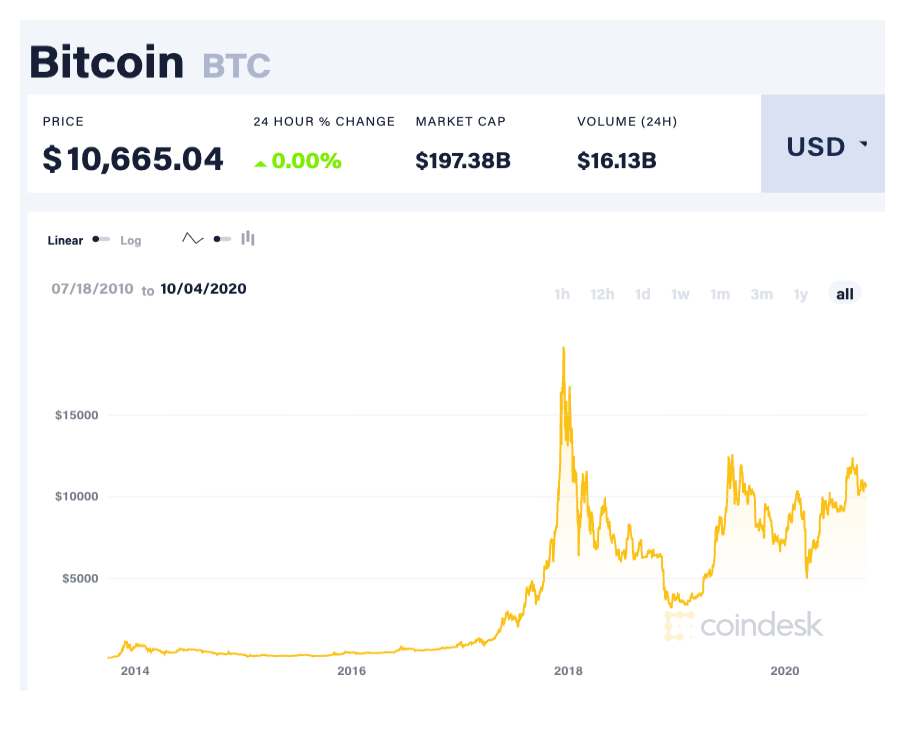
\includegraphics[scale=0.4]{img/btc-chart.png}
  \caption{Preço Histórico do Bitcoin}
  Fonte: https://www.coindesk.com/price/bitcoin
  \label{fig:btc-chart}
\end{figure}

Atualmente, estima-se mais de 375 milhões de dólares sejam comercializados em
bitcoin em apenas um dia.

\subsection{\textit{Machine Learning}}

Segundo \cite{kelleher2020fundamentals}, Machine Learning pode ser definido como 
a automação de processos que extraem padrões dos dados. Compreende um conjunto 
de técnicas computacionais que têm a característica de "aprender" com os dados.

De acordo com \cite{tanaka:2018}, existem três tipos de algoritmos de 
\textit{Machine Learning}:

\begin{itemize}
  \item \textbf{Supervisionado}: Quando se diz ao algoritmo o que é cada entrada 
  (rótulo) e ele aprende quais são as características que influenciam a entrada
  a ser o que ela é.
  \item \textbf{Não supervisionado}: Quando não se diz ao algoritmo o que é cada
  entrada, ou seja, os dados não são rotulados. O algoritmo classifica as 
  entradas conforme suas características semelhantes.
  \item \textbf{Por reforço}: Define-se um sistema de recompensas e punições aos 
  possíveis resultados para que o algoritmo possa ponderar as escolhas a serem 
  feitas.
\end{itemize}

\subsection{Redes Neurais Artificiais}

Redes Neurais Artificiais (RNAs), São modelos matemáticos, compostos por 
unidades de processamentos simples, que calculam determinadas funções 
matemáticas. Uma rede neural artificial é um modelo de computação inspirado na 
forma como a estrutura do cérebro dos mamíferos processa informação 
\cite{de2003tecnicas}.

As unidades de processamento, também chamadas de nós ou neurônios, são
dispostas em uma ou várias camadas e interligadas por conexões. 
As conexões estãoligadas a pesos, que ponderam os valores recebidos por cada 
neurônio.

O conhecimento sobre o problema em consideração está guardado dentro dos
exemplos que têm que estar obrigatoriamente disponíveis. O algoritmo de
aprendizagem generaliza esses dados e memoriza o conhecimento dentro dos
parâmetros adaptáveis da rede, os pesos \cite{rauber2005redes}.

A camada que recebe os dados é chamada de camada de entrada, a camada de saída
é responsável por traduzir o resultado da RNA e quaisquer outras são denominadas 
de camadas ocultas, ou intermediárias, vide Figura \ref{fig:nnet} abaixo. 
Em cada uma das camadas é aplicada uma função de ativação. Durante a fase de 
treinamento, a RNA "aprende" ajustando-se os pesos \cite{bishop1996neural}.

\begin{figure}[ht]
  \centering
  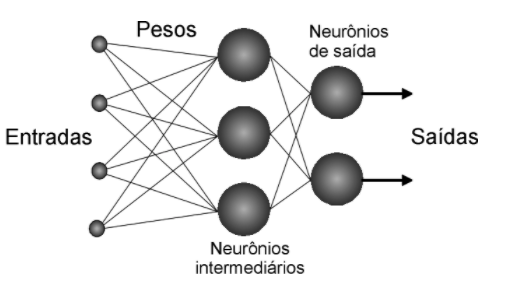
\includegraphics[scale=0.6]{img/nnet.png}
  \caption{Exemplo de uma Rede Neural Artificial de 2 camadas com 4 
  entradas e 2 saídas}
  Fonte: \url{https://cerebromente.org.br/n05/tecnologia/rna.htm}, 
  \\consulta em 02 de outubro de 2020
  \label{fig:nnet}
\end{figure}

\subsubsection{Multilayer Perceptron}

A \textit{Multilayer Perceptron} (MLP), ou Perceptron de Múltiplas Camadas em tradução
direta, é um tipo de Rede Neural artificial que possui mais de uma camada de 
neurônios, interligados em alimentação direta. Uma introdução às Redes Neurais e
Perceptrons pode ser vista em \cite{bailer2001introduction}, mais detalhes sobre
a MLP em \cite{sarle1994neural} e sobre a alimentação direta em 
\cite{bishop1995neural}.

A Figura \ref{fig:mlp} esquematiza uma MLP com duas camadas ocultas:

\begin{figure}[ht]
  \centering
  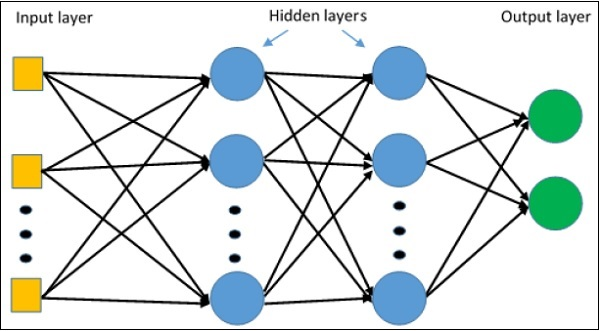
\includegraphics[scale=0.6]{img/multi_layer_perceptron.jpg}
  \caption{
    Exemplo de uma MLP com duas camadas ocultas
  }
  Fonte: \url{https://www.tutorialspoint.com/tensorflow/tensorflow_multi_layer_perceptron_learning.htm}, 
  \\consulta em 02 de outubro de 2020
  \label{fig:mlp}
\end{figure}

\subsection{Regressão Linear Múltipla}

Modelos de regressão linear, assumem que existem uma relação linear entre uma 
variável $y$ (também chamada de variável dependente) e $p$ variáveis independentes
(ou preditoras) \cite{rodrigues2012modelo}. O modelo de regressão linear múltipla é definido 
conforme abaixo:

\begin{equation}
  y_i = \beta_0 + \beta_1x_{i1} + \beta_2x_{i2} + \cdots + \beta_px_{ip} + 
  \varepsilon_i, i = 1, \cdots, n
\end{equation}
em que

\begin{itemize}
  \item $y_i$ é o valor da variável dependente na observação $i$, $i = 1, \cdots, n$;
  \item $x_{ip}$ é o valor da $i$-ésima observação da $p$-ésima variável independente;
  \item $\beta_p$ são os coeficientes da regressão;
  \item $\varepsilon_i$ é o erro aleatório na $i$-ésima observação.
\end{itemize}

Os coeficientes $\beta_j$ representam a média esperada na 
variável resposta $Y$, quando a variável $X_j$ sofre um acréscimo unitário, 
enquanto todas as outras $X_k, k \neq j$ são mantidas constantes.

O coeficiente $\beta_0$ corresponde ao intercepto do plano de regressão. Se o 
modelo incluir $X_j = 0$, então $\beta_0$ será a média de $Y$ nesse ponto.
Caso contrário, não existe interpretação prática para $\beta_0$


\subsection{Random Forests}

Os Random Forests (ou floresta aleatório em tradução direta) é um algoritmo de 
aprendizado de máquina, proposto por \cite{breiman2001random}, que consiste na
geração de diversas árvores de decisão, baseadas em seleções aleatórias e 
variáveis. Após, é realizada uma "votação" entre os modelos e a decisão mais 
votada é a resposta do algoritmo.

É dado pelo modelo:

\begin{equation}
  h(\mathbf{x},\Theta_k), k = 1, \cdots, p
\end{equation}
em que $\Theta_k$ são vetores aleatórios $iid$ e cada árvore, vota para a classe
mais popular da entrada $\mathbf{x}$.

\section{Discussão dos resultados}

A proposta deste artigo é a criação de modelos que consiga entender o
comportamento do preço do Bitcoin e fazer projeções para auxiliar a tomada de
decisões de compra e venda, com o intuito de otimizar os resultados dos 
\textit{trades}.

O primeiro passo para o desenvolvimento deste modelo foi a coleta de dados, 
através da API da corretora \textit{Bitfinex}, e que armazenava o preço do 
Bitcoin, entre outras informações, a cada dez segundos.

Na tabela \ref{summary} é possível verificar algumas estatísticas acerca do 
conjunto de dados.


% Table created by stargazer v.5.2.2 by Marek Hlavac, Harvard University. E-mail: hlavac at fas.harvard.edu
% Date and time: Sun, Oct 04, 2020 - 18:55:22
\begin{table}[!htbp] \centering 
  \caption{Sumarização dos dados} 
  \label{summary} 
\scriptsize 
\begin{tabular}{@{\extracolsep{5pt}} ccccccc} 
\\[-1.8ex]\hline 
\hline \\[-1.8ex] 
 & Min.    & 1st Qu. & Median  & Mean    & 3rd Qu. & Max.    \\ 
\hline \\[-1.8ex] 
     AIL &  3278   &  6384   &  7797   &  7917   &  9442   & 19891   \\ 
     AQ1 &  3561   &  6890   &  8217   &  8456   &  9877   & 20542   \\ 
     AMD &  3706   &  7838   &  8889   &  9357   & 11202   & 22125   \\ 
     AQ3 &  3874   &  8442   & 10762   & 11031   & 12926   & 25195   \\ 
     ASL &  4219   &  9371   & 13501   & 14550   & 19359   & 36100   \\ 
     BIL &     0   &  1783   &  4111   &  4511   &  7300   & 10475   \\ 
     BQ1 &  1001   &  4350   &  6108   &  6110   &  7863   & 13026   \\ 
     BMD &  2822   &  5448   &  6979   &  6917   &  8528   & 16156   \\ 
     BQ3 &  3067   &  5977   &  7412   &  7437   &  9097   & 18124   \\ 
     BSL &  3278   &  6384   &  7797   &  7916   &  9441   & 19890   \\ 
   BAMOUNT &    789.5   &   3785.3   &   9342.7   & 141543.1   & 129697.3   & 835193.2   \\ 
   AAMOUNT &   923.5   &  4961.4   &  7571.0   &  7961.8   & 10788.1   & 20640.8   \\ 
     Bid &  3278   &  6384   &  7797   &  7916   &  9441   & 19890   \\ 
     Ask &   3278   &   6384   &   7797   &   7918   &   9442   & 800000   \\ 
     Last &  3278   &  6384   &  7797   &  7916   &  9442   & 19891   \\ 
     Low &     0   &  6252   &  7502   &  7644   &  9183   & 18734   \\ 
     High &     0   &  6519   &  8049   &  8169   &  9725   & 19891   \\ 
    Volume &      0   &   7102   &  13983   &  23613   &  31641   & 213851   \\ 
   datetime & 2017-11-22 22 & 2018-06-25 11 & 2019-02-11 10 & 2019-01-31 06 & 2019-09-06 16 & 2020-09-29 02 \\ 
\hline \\[-1.8ex] 
\multicolumn{7}{l}{Fonte: Dados do estudo} \\ 
\end{tabular} 
\end{table} 


Apresenta-se na Figura \ref{fig:data-hist} abaixo, a variação do preço do 
Bitcoin, desde o início da coleta dos dados até o momento da elaboração deste 
estudo. Pode-se perceber que no final do ano de 2018, o preço do Bitcoin atingiu 
seu pico máximo, chegando a quase 20 mil dólares. Após um longo período de 
queda, no primeiro semestre do ano de 2019, o preço aumentou consideravelmente, 
chegando a cerca de 13 mil dólares.


\begin{figure}[ht]
  \centering
  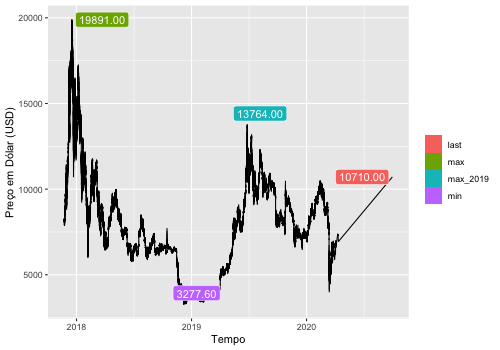
\includegraphics[scale = 0.8]{img/data-hist.pdf}
  \caption{Evolução do preço do Bitcoin, extraído da API da \textit{Bitfinex}}
  Fonte: Dados do estudo
  \label{fig:data-hist}
\end{figure}


Outro ponto relevante que se observa, é um grande gap entre os meses de 
abril e outubro de 2020. Esse fato se deu, por problemas na aplicação que 
consome os dados. Por isso, serão descartados os registros superiores ao mês 
de abril/2020.

O próximo passo foi fazer uma análise das informações que foram coletadas. 
Durante o processo de estruturação do programa que iria fazer a coleta dos 
dados, observou-se que as vezes a API apresentava oscilações de performance, 
ou seja, demorando muitopara retornar o resultado da solicitação.

Verificou-se então a diferença entre cada período coletado. Verifica-se,
Tabela \ref{lag} que existem sete registros com diferença superior a um dia. 

%\clearpage  % Este comando usar com sabedoria você deve, Padawn!

% Table created by stargazer v.5.2.2 by Marek Hlavac, Harvard University. E-mail: hlavac at fas.harvard.edu
% Date and time: Mon, Oct 12, 2020 - 17:42:22
\begin{table}[h] \centering 
  \caption{ \textit{Lag} entre os registros} 
  \label{lag} 
\small 
\begin{tabular}{@{\extracolsep{5pt}} cccc} 
\\[-1.8ex]\hline 
\hline \\[-1.8ex] 
 & Data Final & Data Inicial & Diferença \\ 
\hline \\[-1.8ex] 
1 & 2020-09-29 02:24:54 & 2020-04-11 02:26:54 & 4103:58:00.27338 \\ 
2 & 2018-12-29 16:01:59 & 2018-12-14 10:53:04 & 365:08:55.01703 \\ 
3 & 2020-04-08 20:43:17 & 2020-04-04 04:09:28 & 112:33:48.94099 \\ 
4 & 2019-01-01 21:07:53 & 2018-12-29 17:28:01 & 75:39:51.56921 \\ 
5 & 2020-04-01 02:25:02 & 2020-03-29 21:13:41 & 53:11:21.09238 \\ 
6 & 2020-04-11 02:25:10 & 2020-04-09 02:46:24 & 47:38:46.28917 \\ 
7 & 2020-03-29 20:34:06 & 2020-03-28 14:00:28 & 30:33:37.74005 \\ 
8 & 2020-04-03 02:25:00 & 2020-04-02 03:52:29 & 22:32:30.92597 \\ 
9 & 2020-04-04 02:24:55 & 2020-04-03 05:42:33 & 20:42:22.44385 \\ 
10 & 2019-01-07 14:15:12 & 2019-01-07 07:00:10 & 07:15:01.36821 \\ 
\hline \\[-1.8ex] 
\multicolumn{4}{l}{Fonte: Dados do estudo} \\ 
\end{tabular} 
\end{table} 


Essa primeira análise, subsidiou a decisão de que, apesar dos dados serem 
coletados a cada dez segundos, o modelo confeccionado analisará o período de 
um dia, ou seja, o modelo irá projetar, com base nas informações atuais, 
o preço do bitcoin no práximo dia.

Com isso, o terceiro passo adotado foi filtrar os dados, obedecendo o período 
de um dia. Com isso, o gráfico do preço histório ficou Figura \ref{fig:dataset}
abaixo.

\begin{figure}[!ht]
  \centering
  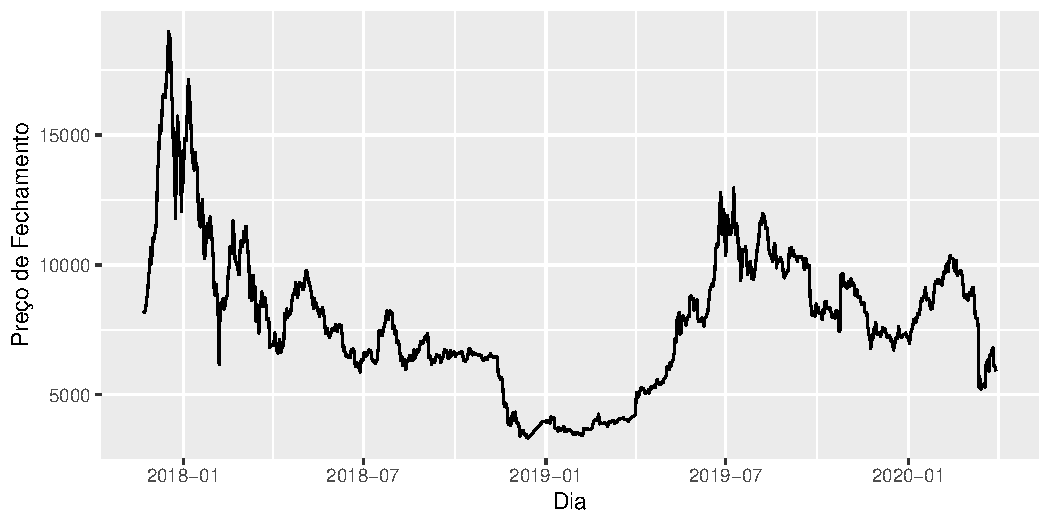
\includegraphics[scale = 0.7]{img/dataset.pdf}
  \caption{Evolução do preço do Bitcoin, após filtros}
  Fonte: Dados do estudo
  \label{fig:dataset}
\end{figure}


Após, prosseguiu-se com a geração das bases de treinamento e teste. Utilizou-se 
como base de treinamento o período compreendido entre 01/11/2017 e 31/12/2019 e
como base de testes o período entre 01/01/2020 a 31/03/2020. Normalizou-se as 
variáveis para todas ficarem compreendidas no intervalo entre menos um e um. 

Executou-se os modelos de Regressão (\textit{lr}) e \textit{Random Forests} 
(\textit{rf}), removendo as variáveis autocorrelacionadas e para o MLP 
(\textit{nn}), utilizou-se todas as variáveis na camada de entrada, considerando 
16 camadas ocultas com 32 neurônios cada e 100 épocas para o treinamento.

Na Figura \ref{fig:results_scatter} abaixo, é possível observar o comparativo
entre o preço previsto (no eixo x) e o preço real (no eixo y), dos modelos 
aplicados na base de testes. Para facilitar a interpretação, foi desenhada uma 
linha tracejada vermelha, onde se lê que quanto mais próximos os pontos estiverem
desta linha, mais preciso será o modelo.

\begin{figure}[!ht]
  \centering
  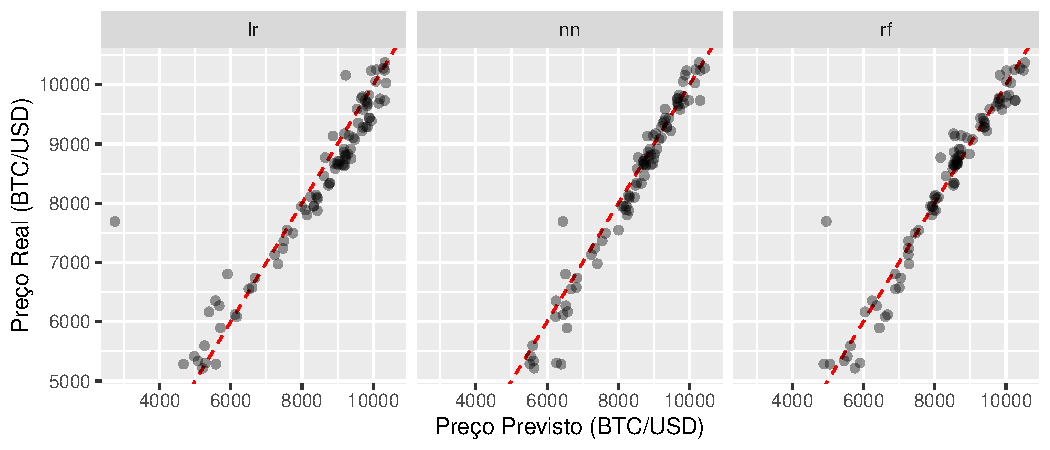
\includegraphics[scale = 0.8]{img/results_scatter.pdf}
  \caption{Evolução do preço do Bitcoin, após filtros}
  Fonte: Dados do estudo
  \label{fig:results_scatter}
\end{figure}


Na figura \ref{fig:results_line}, pode-se analisar os valores previstos (em vermelho)
e reais (em azul) através do tempo. Detaca-se o modelo de Regressão Linear (lr)
que não conseguir prever muito bem os valores em meados do mês de março, enquanto
os modelos Random Forest (rf) e MLP (nn) conseguiram ser mais aderentes nas 
previsões realizadas.


\begin{figure}[!ht]
  \centering
  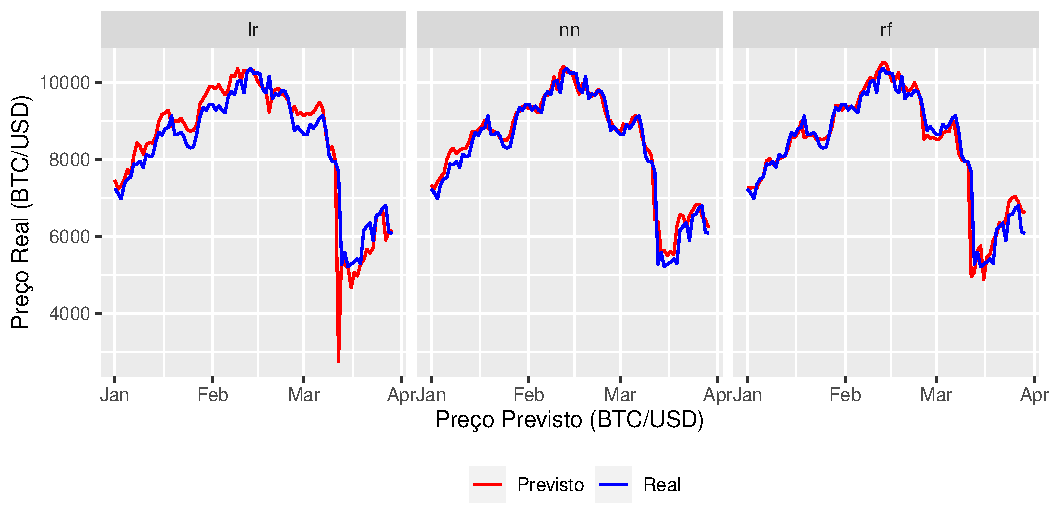
\includegraphics[scale = 0.8]{img/results_line.pdf}
  \caption{Evolução do preço do Bitcoin, após filtros}
  Fonte: Dados do estudo
  \label{fig:results_line}
\end{figure}



Já na tabela \ref{results}, são apresentadas as métricas \textit{Root Mean 
Squared Error} (rmse), $R^{2}$ (rsq) e \textit{Mean Absolute Error} (mae). Para o 
rmse e mae, quanto menor os valores observados, melhor o desenpenho do modelo e 
para o $R^{2}$, quanto maior, melhor.

Com isso, pode-se observar que, confirmando a tendência observada nas Figuras 
\ref{fig:results_scatter} e \ref{fig:results_line}, o modelo de Regressão Linear
Múltipla, apresentou a pior performance os três, quando o modelo \textit{Multilayer
Perceptron}, apresentou ou melhores resultados.


% Table created by stargazer v.5.2.2 by Marek Hlavac, Harvard University. E-mail: hlavac at fas.harvard.edu
% Date and time: Mon, Oct 12, 2020 - 16:30:26
\begin{table}[!htbp] \centering 
  \caption{Métricas dos modelos} 
  \label{results} 
\small 
\begin{tabular}{@{\extracolsep{5pt}} cccc} 
\\[-1.8ex]\hline 
\hline \\[-1.8ex] 
 & lr & nn & rf \\ 
\hline \\[-1.8ex] 
rmse & $642.854$ & $302.027$ & $381.754$ \\ 
rsq & $0.864$ & $0.963$ & $0.928$ \\ 
mae & $360.761$ & $214.231$ & $213.004$ \\ 
\hline \\[-1.8ex] 
\multicolumn{4}{l}{Fonte: Dados do estudo} \\ 
\end{tabular} 
\end{table} 


\section{Considerações finais}

O Objetivo deste trabalho foi implementar e testar modelos capazes de analisar 
dados históricos das cotações do Bitcoin, para identificar o comportamento do 
preço e projetar as cotações futuras.

Construiu-se então três modelos (Regressão Linear Múltipla, \textit{Random Forest}
e \textit{Multilayer Perceptron}), para auxiliar na tomada de decisões e 
estratégias de investimentos em Bitcoin. 

Os resultados mostram que, o modelo \textit{Multilayer Perceptron} conseguiu se
ajustar às variações do preço da moeda de forma mais eficiente que os demais, 
tornando uma ferramenta viável para auxiliar na definição de estratégia de 
investimento.

Outro ponto a ser destacado é que, devido à variação do cenário econômico e outros
quesitos que influenciam o mercado de cryptomoedas, a constante avaliação e
otimização do modelo, com uso de novos dados, é indispensável para se mantenha
uma ferramenta útil para tomada de decisões.

É recomendável que, caso o valor do Bitcoin se estabilize nos próximos meses, um
novo modelo deva ser construído para que se alcance melhores resultados, inclusive
com a aplicação de outras técnicas. Este modelo deve ser abordado em estudos 
futuros.

Além disso, para que se coloque em prática o conhecimento gerado pelo modelo, é
importante o desenvolvimento de uma ferramenta que automatize o processo de 
tomada de decisões de compra e venda, com base nas projeções geradas pelo modelo.
Esta ferramenta será confeccionada em estudos futuros.

\clearpage

\bibliographystyle{sbc}
\bibliography{tcc-bib}

\end{document}
